\documentclass[a4paper,11pt]{article}

\usepackage[spanish]{babel}
\usepackage[utf8]{inputenc}

\usepackage{amsmath}
\usepackage{siunitx}

\usepackage{graphicx}
\usepackage{float}
\usepackage[font=small,labelfont=bf]{caption}


\title{The Triangulation of Titling Data in Non-Linear Gaussian Fashion via $\rho$ Series\thanks{No procrastination}}
\date{2017\\ December}
\author{John Doe\\ Magic Department\thanks{I am no longer a member of this department}, Richard Miles University 
\and Richard Row, \LaTeX\ Academy}

\begin{document}
\maketitle

\section{Introducción}
\clearpage

\section{Método}

	\subsection{Biblioteca utilizada}
	% Descripción biblioteca pyaudio e implementación en el código de los callbacks
    \clearpage
	
	\subsection{Caracterización placa de sonido}
    % Respuesta en frecuencia (amplitud, fase), piso de ruido,
    % linealidad, problemática de tirar los puntos iniciales, gráfico
    % para describir multiplexado/demulitiplexado

En el presente trabajo utilizamos la placa de sonido \emph{Realtek
"MODELO"} para generación y adquisición de señales.  Para ello
utilizamos el puerto de salida analógica estéreo principal y el puerto
de entrada analógica estéreo \emph{line-in}, respectivamente.

Al adquirir señales estéreo con la placa de sonido, esta multiplexa las
señales de los dos canales en un mismo paquete de datos. En la
\textbf{Figura} \ref{fig:multiplexado} se muestra el paquete de datos
obtenido al ingresar una señal senoidal por uno de los canales de
entrada mientras el otro canal se encuentra conectado a
GND.
Para poder separar las dos señales adquiridas en modo estéro se
implementó una función de demultiplexado que permite manipular por
separado las señales de ambos canales de entrada.  Del mismo modo que
con la señal de entrada, cuando se desea utilizar ambos canales de la
salida estéreo se debe proveer a la placa de sonido un paquete de datos
con las dos señales multiplexadas. Para facilitar la manipulación de esos
datos también implementamos la función de multiplexado respectiva.

    \begin{figure}[!h] 
        \centering
        \includegraphics[width=0.9\textwidth]{imagenes/estereo.pdf}
        \caption{Paquete de datos obtenidos al leer la señal de entrada
estereo cuando un canal se encuentra alimentado por una señal senoidal
mientras el otro canal se encuentra conectado a GND.}
        \label{fig:multiplexado} 
    \end{figure}

Los paquetes de datos que se reciben y se envían a la placa de sonido
contienen la información de la amplitud de las señal traducida a una
unidad de cuentas aribtraria. Para poder establecer la correlación de
esta unidad arbitraria con un valor de tensión realizamos un proceso de
calibración tanto de la entrada como de la salida de la placa de sonido.
Para ello generamos con la placa de sonido señales sinusoidales de
distintas amplitudes, estas señales fueron medidas con un osciloscopio
externo y a su vez fueron ingresadas como entrada a la placa de sonido.
Se registraron los valores de las unidades arbitrarias y su valores de
tensión respectivo con el objetivo de ajustar una curva de calibración
tanto de los canales de entrada como de los canales de salida de la
placa.  En las \textbf{Figuras} \ref{fig:CalibracionEntrada} y
\ref{fig:CalibracionSalida} se muestran las curvas de calibración
obtenidas.  Los datos medidos fueron ajustados linealmente obteniéndose
las siguientes expresiones,
	
\begin{equation*}
	 \text{Tensión de salida} = \SI{1.62}{\V} * Cuentas + \SI{0.108}{\V}
\end{equation*}

\begin{equation*}
	\text{Tensión de entrada} = \SI{2.555}{\V} * Cuentas + \SI{0.09116}{\V}
\end{equation*}

Utilizando las curvas de calibración obtenidas generamos funciones
adicionales que permiten convertir una señal que contiene la información
en cuentas de unidad arbitraria en valores de tensión y viceversa.

	\begin{figure}[!h]
		\centering
		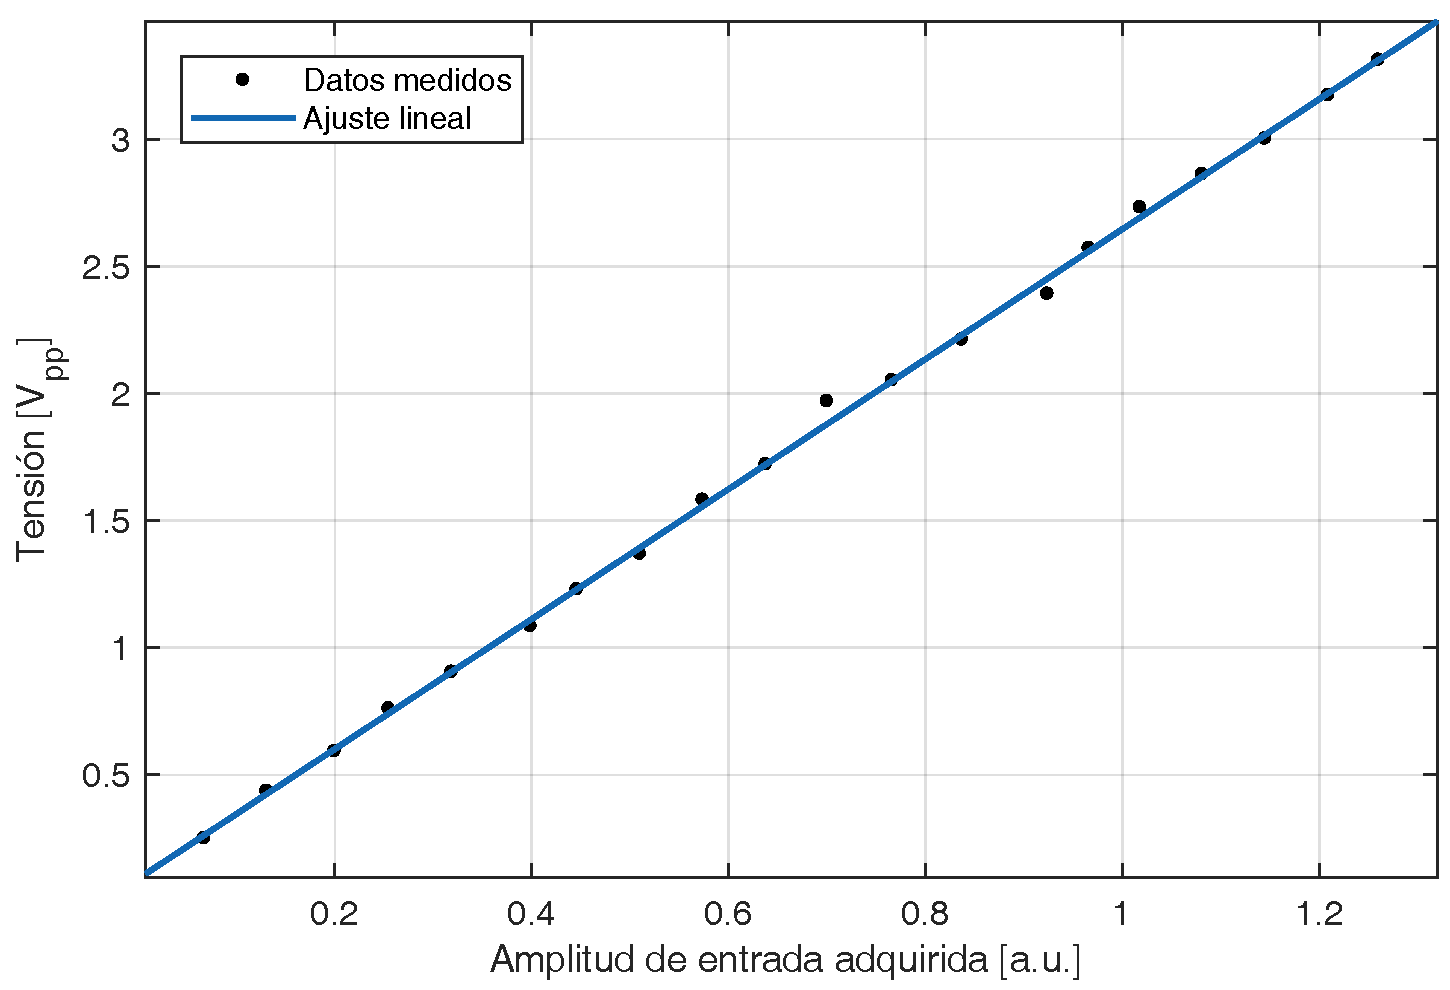
\includegraphics[width=\textwidth]{imagenes/CalibracionEntrada.pdf}
		\caption{Curva de calibración de la señal de entrada de la placa
de sonido.}
        \label{fig:CalibracionEntrada}
	\end{figure}
	
	\begin{figure}[!h]
		\centering
		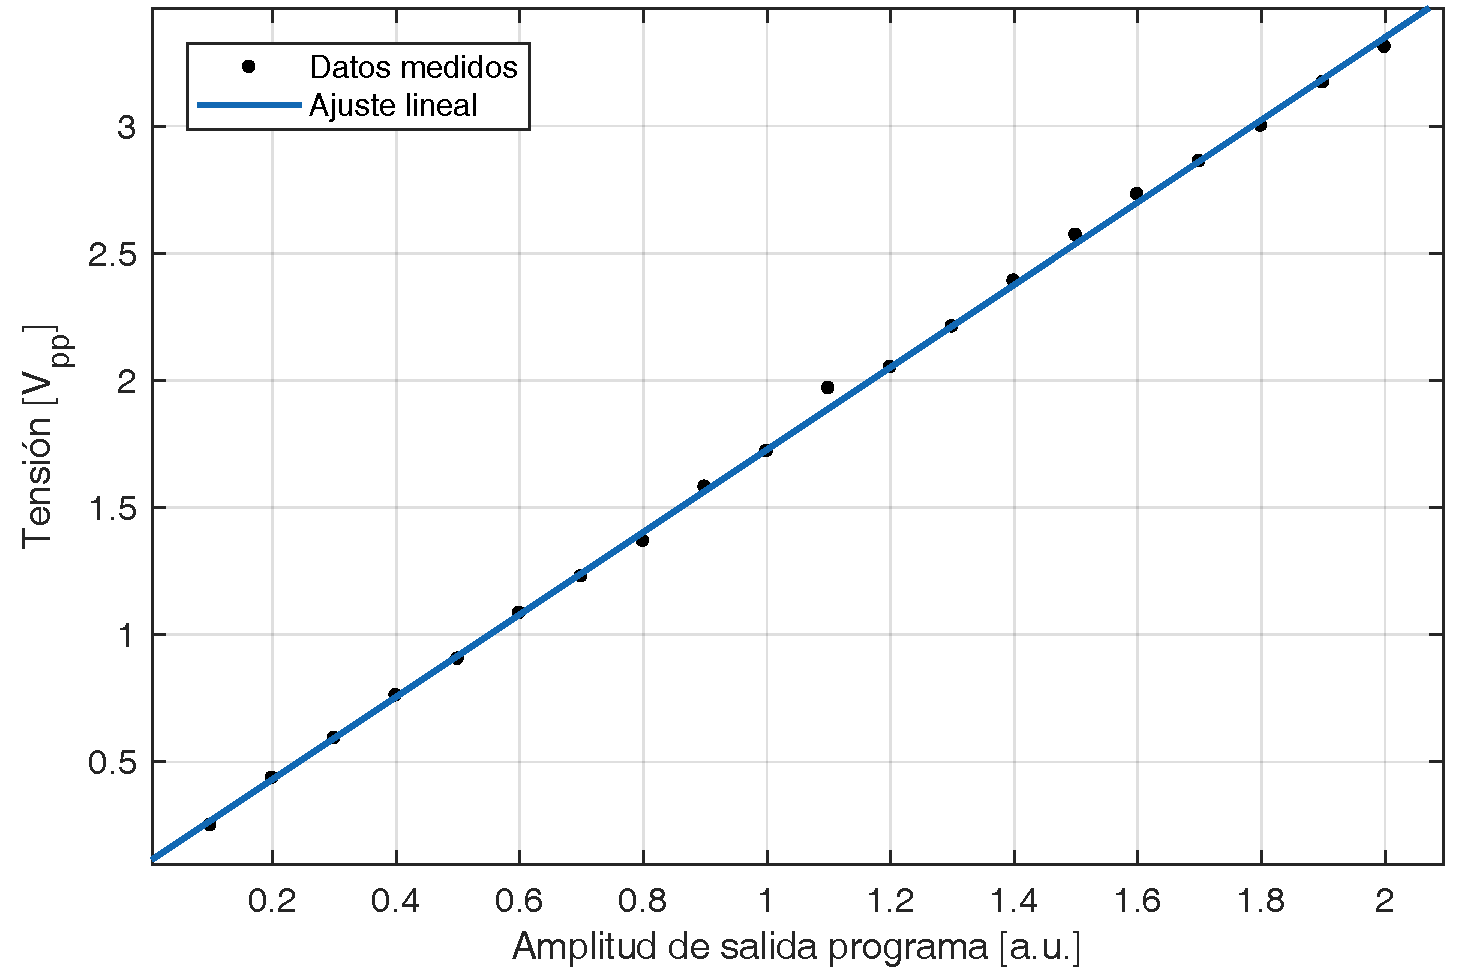
\includegraphics[width=\textwidth]{imagenes/CalibracionSalida.pdf}
		\caption{Curva de calibración de la señal de salida de la placa
de sonido.}
        \label{fig:CalibracionSalida}
	\end{figure}

Para poder caracterizar la respuesta en frencuencia de la placa de
sonido realizamos un barrido en frecuencias generando señales
sinusoidales de distintas frecuencias con la salida de la placa que
fueron ingresada como entrada a la misma. Registramos la variación en la
ganancia del sistema en función de la frecuencia, los resultados se
muestran en las \textbf{Figuras} \ref{fig:bode44k1} y \ref{fig:bode192k}
para dos frecuencias de muestreo distintas.

	\begin{figure}[!h]
		\centering
		\includegraphics[width=0.9\textwidth]{imagenes/bode44k1Hz.png}
		\caption{Variación de la ganancia en función de la frecuencia de
la señal, para una frecuencia de muestreo configurada de \SI{44.1}{\kHz}}
        \label{fig:bode44k1}
	\end{figure}

	\begin{figure}[!h]
		\centering
		\includegraphics[width=0.9\textwidth]{imagenes/bode192kHz.png}
		\caption{Variación de la ganancia en función de la frecuencia de
la señal, para una frecuencia de muestreo configurada de \SI{192}{\kHz}}
        \label{fig:bode192k}
	\end{figure}

Para poder establecer el mínimo valor de señal de tensión que puede
registrarse con la placa de sonido medimos el piso de rudio de la misma.
Conectamos ambos canales de la entrada estéreo a GND y registramos la
señal obtenida, los resultados para cada canal se muestran en las
\textbf{Figuras} \ref{fig:RuidoIzquierdo} y \ref{fig:RuidoDerecho}.
El valor del rudio RMS obtenido es de $\SI{277}{\uV}$.

	\begin{figure}[h]
		\centering
		\includegraphics[width=0.9\textwidth]{imagenes/RuidoCanalIzquierdo.png}
		\caption{Señal de ruido correspondiente al canal izquierdo del
puerto de entrada estéreo.}
        \label{fig:RuidoIzquierdo}
	\end{figure}
	
	\begin{figure}[h]
		\centering
		\includegraphics[width=0.9\textwidth]{imagenes/RuidoCanalDerecho.png}
		\caption{Señal de ruido correspondiente al canal derecho del
puerto de entrada estéreo.}
        \label{fig:RuidoDerecho}
	\end{figure}
\clearpage

\section{Resultados}

	\subsection{Discreto}
	% Curva I-V
	
	\begin{figure}[h]
		\centering
		\includegraphics[width=\textwidth]{imagenes/Diodo1N4148.png}
		\caption{}
	\end{figure}
	
	\subsection{Integrado}
	

\end{document}
